\documentclass[a4paper]{article}
%\usepackage{amsfonts}
\usepackage{amsmath}
%\usepackage{amsthm}
\usepackage[utf8]{inputenc}
%\usepackage{hyperref}
%\usepackage{booktabs}
\usepackage{graphicx}
\usepackage{subfig}

\title{Exercises on physical design}
\author{Rodrigo Arias Mallo}
\date{\today}

\newcommand*\mat[1]{ \begin{pmatrix} #1 \end{pmatrix}}
\newcommand*\arr[1]{ \begin{bmatrix} #1 \end{bmatrix}}
\newcommand*\V[1]{ \boldsymbol{#1}}

\begin{document}
\maketitle

\section{Quadratic placement}

% A = [[ 3 -1 -1  0]
%  [-1  3  0 -1]
%  [-1  0  2  0]
%  [ 0 -1  0  2]]
% bx = [ 2.  0.  4.  4.]
% by = [ 0.  4.  3.  3.]
% X = [ 2.28571429  1.71428571  3.14285714  2.85714286]
% Y = [ 1.76190476  2.9047619   2.38095238  2.95238095]

By computing the Laplacian matrix of the graph, and removing the rows and 
columns of the fixed cells, we get the matrix $A$ used in the linear equation 
system.
%
$$ A = \mat{
	 3 & -1 & -1 &  0 \\
	-1 &  3 &  0 & -1 \\
	-1 &  0 &  2 &  0 \\
	 0 & -1 &  0 &  2}$$
%
The right hand side for $x$ is $b^x = \mat{2 & 0 & 4 & 4}^T$ and for $y$ is $b^y 
= \mat{0 & 4 & 3 & 3}^T$, so we can solve now the two systems: $AX = b^x$ and 
$AY = b^y$ and obtain the coordinates of the non-fixed cells.
%
$$ X = \mat{2.29 & 1.71 & 3.14 & 2.86}^T,\quad
Y = \mat{1.76 & 2.90 & 2.38 & 2.95}^T $$
%
The graph can be plotted now, where the black nodes are the fixed ones 
$\{u,v,w\}$ while the gray nodes are the non-fixed cells $\{a,b,c,d\}$. For 
details see the python script \texttt{placement.py}.
%
\begin{center}
\includegraphics[width=.7\textwidth]{placement.pdf}
\end{center}
%
\section{Channel routing}

The vertical graph can be computed from the two vectors TOP and BOT.
%
\begin{center}
\includegraphics[width=.5\textwidth]{vertical.pdf}
\end{center}
%
As there are no loops, no conflicts are detected, and the graph corresponds with 
the vertical constraint graph with net splitting. The zone representation can be 
computed by first connecting the pins endpoints.
%
\begin{center}
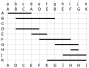
\includegraphics[width=.5\textwidth]{zone.pdf}
\end{center}
%
The set of maximal nets are %
$S(d) = \{A,B,D,E\}$, %
$S(e)= \{B,D,E,F\}$, %
$S(f)= \{B,E,F,K\}$, %
$S(h)= \{E,F,G,J,K\}$ and %
$S(i)= \{F,G,H,J,K\}$. %
From which we can finally obtain the zone representation.
%
\begin{center}
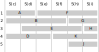
\includegraphics[width=.5\textwidth]{zone2.pdf}
\end{center}
%
So we find that the minimum number of tracks is 5. However, if we split the 
nets, the net $E$ becomes $E_1$ and $E_2$, and the vertical constraint graph
%
\begin{center}
\includegraphics[width=.6\textwidth]{vertical-split.pdf}
\end{center}
%
But the same number of minimum tracks is obtained, as can be seen in the zone 
representation:
%
\begin{center}
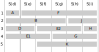
\includegraphics[width=.5\textwidth]{zone-repr-split.pdf}
\end{center}
%
After running the Dogleg Left-Edge algorithm, the routed channel is drawn as 
following.
%
\begin{center}
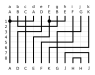
\includegraphics[width=.4\textwidth]{route2.pdf}
\end{center}
%
\newpage

\section{Slicing floorplan}

In order to draw the functions at every node, a number is attached to each H and 
V node, the graph then becomes
%
\begin{center}
\includegraphics[width=.5\textwidth]{floor-graph.pdf}
\end{center}
%
After computing the shape function at each node, we find that the best size is 
8 units of height and 6 units of width, in total 48 units of area.
%
\begin{center}
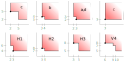
\includegraphics[width=.9\textwidth]{floorplan.pdf}
\end{center}
%
A new floorplan can be obtained which reduces the size to 5 by 9, giving 45 
units of area. Both can be seen in the following picture.
%
\begin{center}
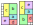
\includegraphics[width=.4\textwidth]{plans.pdf}
\end{center}
%





\end{document}
